\documentclass[12pt,aspectratio=169]{beamer}


\usepackage{algorithm,algorithmic}

\usepackage[utf8]{inputenc}
\usepackage{booktabs}
\usepackage[opacity=0.1]{pdfcomment} % set to 0 to make annotation icons invisible
\usepackage{pdfpc}
\usepackage{arev}
\usepackage{multicol}

\usepackage{xcolor, color, colortbl}
\definecolor{dkgreen}{rgb}{0,0.5,0}
\definecolor{dkred}{rgb}{0.8,0,0}
\definecolor{dkblue}{rgb}{0,0,0.5}
\definecolor{gray}{rgb}{0.5,0.5,0.5}
\definecolor{mauve}{rgb}{0.58,0,0.82}
\definecolor{hilight}{RGB}{122,86,0}

\definecolor{LRed}{rgb}{1,.8,.8}
\definecolor{MRed}{rgb}{1,.6,.6}
\definecolor{HRed}{rgb}{1,.2,.2}

\usepackage{tikz}
\usetikzlibrary{arrows.meta,
                calc, chains,
                quotes,
                positioning,
                shapes.geometric}


\def\scalefact{0.85}
\newcommand{\cev}[1]{\reflectbox{\ensuremath{\vec{\reflectbox{\ensuremath{#1}}}}}}
\newcommand{\evalat}[2]{\left.#1\right\vert_{#2}}

\newcommand{\znode}[5][black]{\path (#3,#4) node(#2) [circle,draw,color=#1] {#5};}
\newcommand{\zunedge}[6][black]{%
\begin{scope}
	\path (#2,#3) node(this) [inner sep=0pt,triangle,draw,color=#1] {#4};
	\draw[->,color=#1] (#5) -- (this.west);
	\draw[->,color=#1] (this.east) -- (#6);
\end{scope}}
\newcommand{\zbiedge}[7][black]{%
\begin{scope}
	\path (#2,#3) node(this) [inner sep=0pt,triangle,draw,color=#1] {#4};
	\draw[->,color=#1] (#5) -- (this);
	\draw[->,color=#1] (#6) -- (this);
	\draw[->,color=#1] (this.east) -- (#7);
\end{scope}}
\newcommand{\zedge}[5][black]{\path (#3,#4) node(#2) [inner sep=0pt,triangle,draw,color=#1] {#5};}

\definecolor{blue(pigment)}{rgb}{0.2, 0.2, 0.6}
\definecolor{burgundy}{rgb}{0.5, 0.0, 0.13}


\usepackage{listings}
%% \usetheme{Goettingen}
\usefonttheme{serif}
\usepackage{times}
\setbeamertemplate{navigation symbols}{}
\title{Deep Learning}
\subtitle{Lecture 4: Perceptron}
 
 
%\author[Mehrdad Maleki] % (optional, for multiple authors)
%{Mehrdad Maleki, Barak A. Pearlmutter\footnote{ Institute & Department of Computer Science
%Maynooth University, Co. Kildare, Ireland}, Jeffrey Mark Siskind}
 
%\institute[NUIM] % (optional)
%{
%  Department of Computer Science \\
%  National University of Ireland Maynooth
 
%}

\author[]{\textbf{Dr. Mehrdad Maleki}}
%\institute[]{\textsuperscript{1}Department of Computer Science\\ National University of Ireland\\ Maynooth}
 
\date{}
 
%\logo{\includegraphics[height=1.5cm]{lion-logo.png}}

\renewcommand{\Re}{\mathbb{R}}
 
\begin{document}
 
\frame{\titlepage}

\newcommand{\SYSTEM}[2]{\raisebox{-1ex}{\shortstack{#1\\[-0.25ex]\tiny #2}}}
\newcommand{\YES}{\textcolor{dkgreen}{$\ballotcheck$}}
\newcommand{\NOPE}{\textcolor{dkred}{$\ballotx$}}
\newcommand{\MAYBE}{\textcolor{dkblue}{\textbf{?}}}



%\begin{frame}
%\frametitle{Backpropagator}
%\begin{figure}[t!]
%\scalebox{\scalefact}{%
%\begin{tikzpicture} [
%    triangle/.style = {regular polygon, regular polygon sides=3,shape border rotate=270 },
%    ]
% % 	\draw[style=help lines] (0,0) grid (14,4);
%	\znode[blue(pigment)]{x1}{0}{1.75}{$x_1$}
%	\znode[blue(pigment)]{x2}{0}{0.25}{$x_2$}
%	\znode[blue(pigment)]{z1}{2}{1}{$z_1$}
%	\znode[blue(pigment)]{z2}{4}{1}{$z_2$}
%	\znode[blue(pigment)]{y}{6.25}{1}{$y$}
%	\zbiedge[blue(pigment)]{0.85}{1}{$\,-\,$}{x1}{x2}{z1}
%	\zedge[blue(pigment)]{mul}{3}{1}{$\ \cdot\ $}
%	\draw[->,color=blue(pigment)] (z1) to[bend left] (mul);
%	\draw[->,color=blue(pigment)] (z1) to[bend right] (mul);
%	\draw[->,color=blue(pigment)] (mul) to (z2);
%	\zunedge[blue(pigment)]{5}{1}{$\sin$}{z2}{y}
%	% The diff part
%	\znode[burgundy]{a}{6.25}{3.75}{$a$}
%	\znode[burgundy]{b}{8}{3}{$b$}
%	\znode[burgundy]{v}{6.25}{2.25}{$v$}
%	\znode[burgundy]{cp}{10}{3.75}{$c'$}
%	\znode[burgundy]{cpp}{10}{2.25}{$c''$}
%	\znode[burgundy]{c}{12}{3}{$c$}
%	\znode[burgundy]{cox1}{14}{3.75}{$x_1'$}
%	\znode[burgundy]{cox2}{14}{2.25}{$x_2'$}
%	\zunedge[burgundy]{5}{2.25}{$\cos$}{z2}{v}
%	\zbiedge[burgundy]{7}{3}{$\ \cdot\ $}{a}{v}{b}
%	\zedge[burgundy]{mul1}{9}{3.75}{$\ \cdot\ $}
%	\draw[->,color=burgundy] (z1) to[out=60,in=200] (5,4) to[out=20,in=160] (mul1);
%	\draw[->,color=burgundy] (b) to (mul1);
%	\draw[->,color=burgundy] (mul1) to (cp);
%	\zedge[burgundy]{mul2}{9}{2.25}{$\ \cdot\ $}
%	\draw[->,color=burgundy] (z1) to[out=315,in=225] (mul2);
%	\draw[->,color=burgundy] (b) to (mul2);
%	\draw[->,color=burgundy] (mul2) to (cpp);
%	\zbiedge[burgundy]{11}{3}{$+$}{cp}{cpp}{c}
%	\znode[burgundy]{one}{12}{4}{$1$}
%	\zedge[burgundy]{mul3}{13}{3.75}{$\ \cdot\ $}
%	\draw[->,color=burgundy] (one) to (mul3);
%	\draw[->,color=burgundy] (c) to (mul3);
%	\draw[->,color=burgundy] (mul3) to (cox1);
%	\znode[burgundy]{negone}{12}{2}{$-1$}
%	\zedge[burgundy]{mul4}{13}{2.25}{$\ \cdot\ $}
%	\draw[->,color=burgundy] (negone) to (mul4);
%	\draw[->,color=burgundy] (c) to (mul4);
%	\draw[->,color=burgundy] (mul4) to (cox2);
%\end{tikzpicture}}
%\textsf{\textcolor{blue}{let} z$_1$=x$_1$-x$_2$ \textcolor{blue}{in let} z$_2$=z$_1\cdot$z$_1$ \textcolor{blue}{in let} b=($\cos$ z$_2$)$\cdot$a \textcolor{blue}{in let} c=z$_1\cdot$b+z$_1\cdot$b \textcolor{blue}{in} ($\sin$ z$_2$,(1$\cdot$c,-1$\cdot$c))}
%\end{figure}
%\pdfpcnote{If memory contains w := (u, a) and z i := (s i , b i )
%for all i, we update the memory with the assignments z i := (s i , b i + D i f (s) · a). 
%x 1 := (5, 0), x 2 := (2, 0), z 1 := (3, 0), z 2 :=
%(9, 0), y := (0.412, 1). From here, the backward phase updates z 2 := (9, cos(z 2 ) · 1) = (9, −0.911),
%then z 1 := (3, z 1 · −0.911 + z 1 · −0.911) = (3, −5.467) and finally x 1 := (5, 1 · −5.467) = (5, −5.467)
%and x 2 := (2, −1 · −5.467) = (2, 5.467)}
%\end{frame}

%
%\begin{frame}
%  \frametitle{Overview}
%  \begin{center}
%  \begin{tabular}{cccccc}\toprule
%    \textbf{System} & \textbf{In-Lang} & \textbf{Nests} & \textbf{HO-Lang} & \textbf{HO-IO} & \textbf{Compile}
%    \\\cmidrule(r){1-1}\cmidrule{2-6}
%    \SYSTEM{ADOLC}{tape}
%    & \YES & \NOPE & \YES & \NOPE & \NOPE
%    \\[1ex]
%    \SYSTEM{R$^6$RS-AD}{tape}
%    & \YES & \YES & \YES & \NOPE & \NOPE
%    \\[1ex]
%    \SYSTEM{Tapenade}{tape}
%    & \NOPE & \NOPE & \NOPE & \NOPE & \YES
%    \\[1ex]
%    \SYSTEM{LtUB}{(Pearlmutter \& Siskind, 2008)}
%    & \YES & \YES & \YES & \YES & \YES
%    \\[1ex]
%    \SYSTEM{DPPL}{(Mak \& Ong, 2020)}
%    & \YES & \MAYBE & \YES & \YES & \NOPE
%    \\[1ex]
%    \SYSTEM{Diff Curry}{(Vytiniotis et al., 2019)}
%    & \NOPE & \NOPE & \YES & \NOPE & \YES
%    \\[1ex]
%    \SYSTEM{Linear Negation}{(Brunel et al., 2019)}
%    & \NOPE & \MAYBE & \YES & \NOPE & \NOPE
%    \\[1ex]
%    \SYSTEM{Simple Diff PL}{(Abadi \& Plotkin, 2020)}
%    & \YES & \MAYBE & \NOPE & \NOPE & \YES
%    \\
%    \bottomrule
%  \end{tabular}
%  \end{center}
%  \vspace{-0.5ex}
%  \begin{tiny}
%    \begin{multicols}{2}
%    \begin{description}
%    \item[System] Name of formalization
%    \item[In-Lang] Diff.\ is in-language operator/syntax
%    \item[Nests] Can nest derivatives
%    \item[HO-Lang] User code in higher-order language
%    \item[HO-IO] Can diff higher-order funcs (e.g., \texttt{map})
%    \item[Compile] Suitable for integration into optimizing compiler
%    \end{description}
%    \end{multicols}
%  \end{tiny}
%  \pdfpcnote{R$^6$RS-AD: These are some AD (Automatic Differentiation) tools for both forward
%and reverse mode written for R6RS Scheme.  They run under Ikarus and
%PLT Scheme. \\Tapenade: is an Automatic Differentiation (AD) tool which, given a Fortran or C code that computes a function,
%creates a new code that computes its tangent or adjoint derivatives. Tapenade puts particular emphasis
%on adjoint differentiation, which computes gradients at a remarkably low cost.}
%\end{frame}

\begin{frame}
  \frametitle{Boolean Functions}
  \begin{large}
    Boolean variable, $X=0$ or $X=1$.\pause
    \bigskip
    \begin{enumerate}
    \item AND: $X\wedge Y=1 \Leftrightarrow X=Y=1$ \pause

      \smallskip

    \item OR: $X\vee Y=1 \Leftrightarrow X=1$ or $Y=1$ \pause

      \smallskip

    \item NEGATION: 
      \begin{align*}
        &\overline{X}=1 \Leftrightarrow X=0\\
        &\overline{X}=0 \Leftrightarrow X=1
      \end{align*}
      \pause
       \smallskip
       
      \item XOR: $X \oplus Y=(\overline{X}\wedge Y)\vee (X \wedge \overline{Y})$
      
    \end{enumerate}
      \end{large}
\end{frame}

\begin{frame}
\frametitle{Some useful properties}
\begin{itemize}
\item $\overline{X\wedge Y}=\overline{X}\vee \overline{Y}$\pause
\bigskip
\item $\overline{X\vee Y}=\overline{X}\wedge \overline{Y}$\pause
\bigskip
\item $\overline{\overline{X}}=X$
\end{itemize}
\end{frame}

\begin{frame}
%\begin{center}
%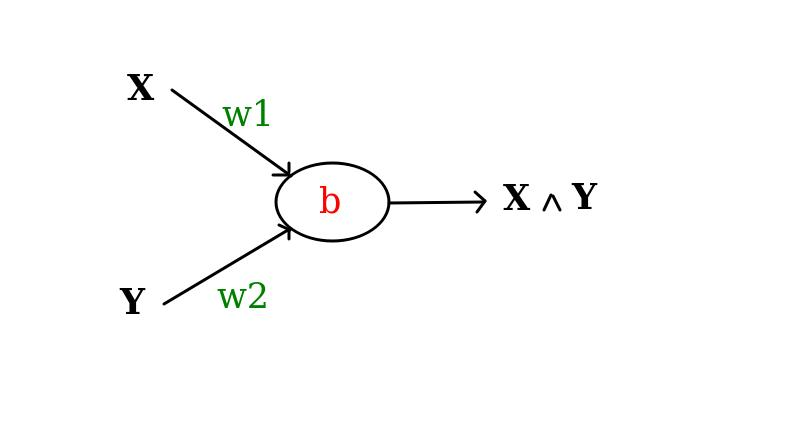
\includegraphics[scale=0.6]{and}
%\end{center}

\begin{figure}
\begin{tikzpicture}
\draw[blue,ultra thick]  (3,0) circle (20pt);
\foreach \y in {2,-2}
  \draw[->] (0,\y) -- (2.3,0);
\foreach \y/\x in{2/$X$,-2/$Y$}
  \node[left] at (0,\y) {\x};

\foreach \y/\x in{2/$w_1$,-1.5/$w_2$}
  \node[above,orange] at (0+0.9,\y-0.5) {\x};

\draw[->] (3.7,0) -- (5,0);

\node[right,brown] at (5,0) {$X\wedge Y$};
\node[red] at (3,0) {$b$};
\end{tikzpicture}
\end{figure}


\[
X \wedge Y=\left \{ \begin{array}{ll}
1 &\mbox{if }w_1*X+w_2*Y\geq b\\
0 &\mbox{else}
\end{array}
\right.
\]
\end{frame}

\begin{frame}
\[
\begin{aligned}
& 1\wedge 1=1 \Rightarrow w_1+w_2\geq b\\
& 1\wedge 0=0 \Rightarrow w_1< b\\
& 0\wedge 1=0 \Rightarrow w_2< b\\
& 0\wedge 0=0 \Rightarrow 0< b
\end{aligned}
\]
find integers $w_1,w_2,b$ that satisfies all of these constraints.
\end{frame}

\begin{frame}
\begin{figure}
\begin{tikzpicture}[thick,fill opacity=.3,draw opacity=3]
\draw[->] (0,-1) -- (0,5);
\draw[->] (-5,0) -- (5,0);
\node[right] at (5,0) {$w_1$};
\node[left] at (0,5) {$w_2$};
\draw[red] (-1,3) -- (3,-1);
\node[left] at (0,2) {$2$};
\node[below] at (2,0) {$2$};
\draw[fill=pink, draw=none,rotate around={45:(3,-1)}] (3,-1) rectangle (8,5);\pause

\draw[fill=green, draw=none] (-1,-1) rectangle (8,2);
\draw[dotted] (-1,2)-- (6,2); \pause
\draw[fill=green, draw=none] (-1,-1) rectangle (2,7);
\draw[dotted] (2,-1)-- (2,6); \pause
\node[above] at (2,2) {$(2,2)$};\pause
\draw[dotted, fill=blue] (2,0) -- (2,2) -- (0,2) -- cycle;
\draw[] (2,0) -- (0,2);\pause
\node[below] at (1,1) {$(1,1)$};
\fill[] (1,1) circle [radius=2pt];
\end{tikzpicture}
\end{figure}
\end{frame}

%
%\begin{frame}
%\begin{center}
%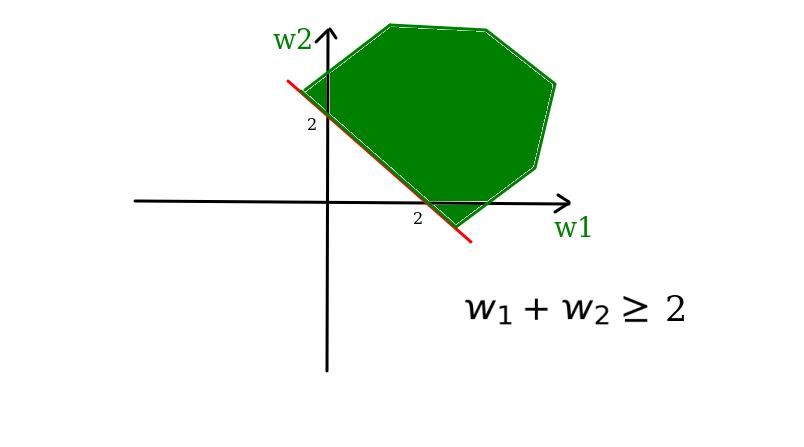
\includegraphics[scale=0.6]{and3}
%\end{center}
%\end{frame}

%
%\begin{frame}
%\begin{center}
%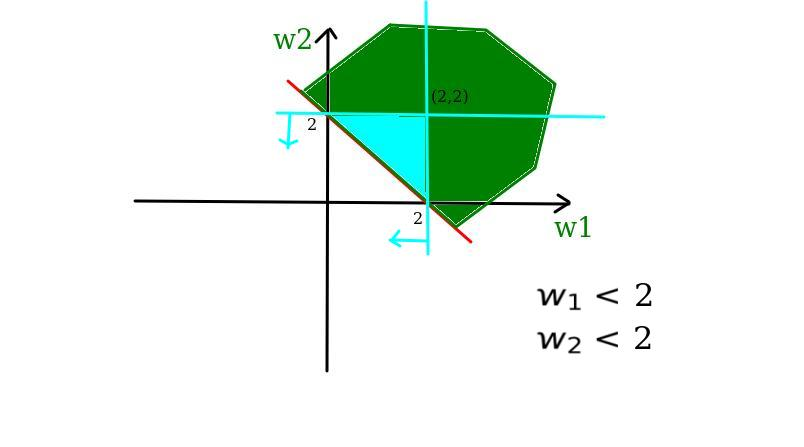
\includegraphics[scale=0.6]{and4}
%\end{center}
%\end{frame}
%
%
%\begin{frame}
%\begin{center}
%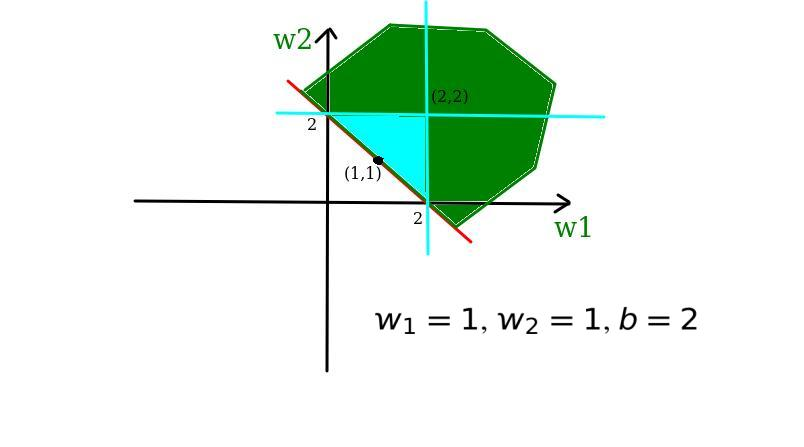
\includegraphics[scale=0.6]{and5}
%\end{center}
%\end{frame}



\begin{frame}
%\begin{center}
%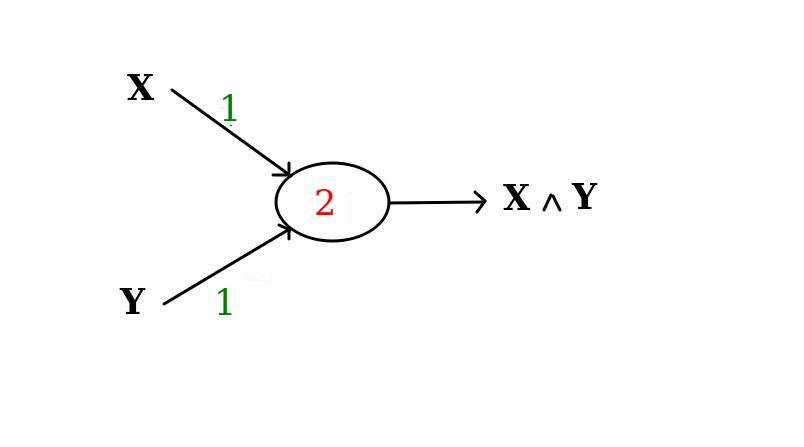
\includegraphics[scale=0.6]{and2}
%\end{center}

\begin{figure}
\begin{tikzpicture}
\draw[blue,ultra thick]  (3,0) circle (20pt);
\foreach \y in {2,-2}
  \draw[->] (0,\y) -- (2.3,0);
\foreach \y/\x in{2/$X$,-2/$Y$}
  \node[left] at (0,\y) {\x};

\foreach \y/\x in{2/$1$,-1.5/$1$}
  \node[above,orange] at (0+0.9,\y-0.5) {\x};

\draw[->] (3.7,0) -- (5,0);

\node[right,brown] at (5,0) {$X\wedge Y$};
\node[red] at (3,0) {$2$};
\end{tikzpicture}
\end{figure}


\[
X \wedge Y=\left \{ \begin{array}{ll}
1 &\mbox{if }X+Y\geq 2\\
0 &\mbox{else}
\end{array}
\right.
\]
\end{frame}
%-------

\begin{frame}
%\begin{center}
%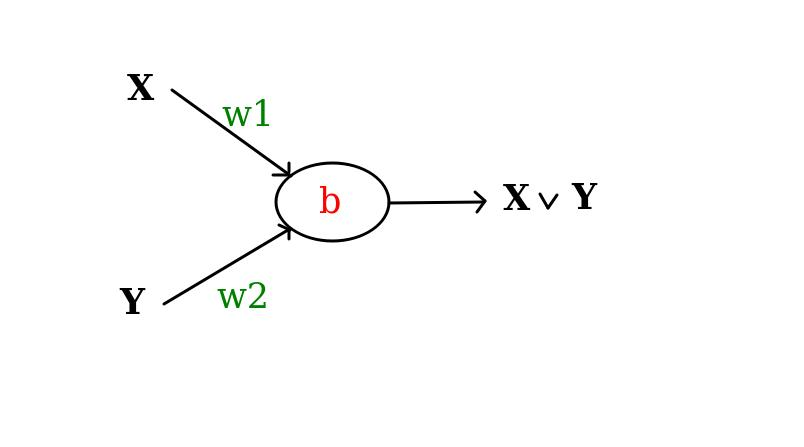
\includegraphics[scale=0.6]{or}
%\end{center}

\begin{figure}
\begin{tikzpicture}
\draw[blue,ultra thick]  (3,0) circle (20pt);
\foreach \y in {2,-2}
  \draw[->] (0,\y) -- (2.3,0);
\foreach \y/\x in{2/$X$,-2/$Y$}
  \node[left] at (0,\y) {\x};

\foreach \y/\x in{2/$w_1$,-1.5/$w_2$}
  \node[above,orange] at (0+0.9,\y-0.5) {\x};

\draw[->] (3.7,0) -- (5,0);

\node[right,brown] at (5,0) {$X\vee Y$};
\node[red] at (3,0) {$b$};
\end{tikzpicture}
\end{figure}


\[
X \vee Y=\left \{ \begin{array}{ll}
1 &\mbox{if }w_1X+w_2Y\geq b\\
0 &\mbox{else}
\end{array}
\right.
\]
\end{frame}
%
\begin{frame}
%\begin{center}
%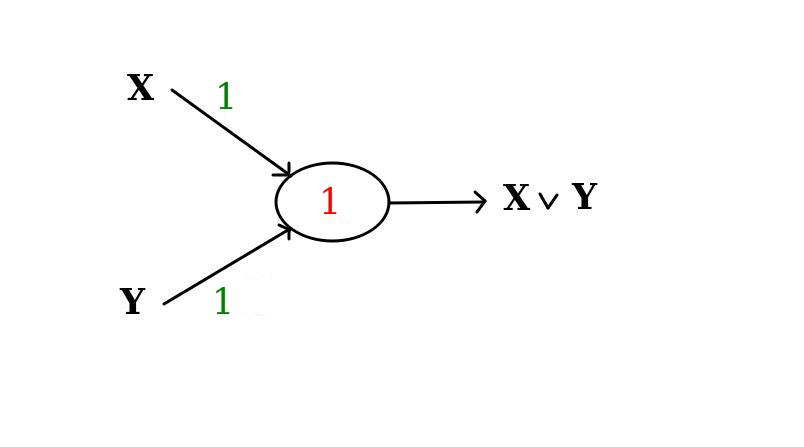
\includegraphics[scale=0.6]{or2}
%\end{center}
\begin{figure}
\begin{tikzpicture}
\draw[blue,ultra thick]  (3,0) circle (20pt);
\foreach \y in {2,-2}
  \draw[->] (0,\y) -- (2.3,0);
\foreach \y/\x in{2/$X$,-2/$Y$}
  \node[left] at (0,\y) {\x};

\foreach \y/\x in{2/$1$,-1.5/$1$}
  \node[above,orange] at (0+0.9,\y-0.5) {\x};

\draw[->] (3.7,0) -- (5,0);

\node[right,brown] at (5,0) {$X\vee Y$};
\node[red] at (3,0) {$1$};
\end{tikzpicture}
\end{figure}

\[
X \vee Y=\left \{ \begin{array}{ll}
1 &\mbox{if }X+Y\geq 1\\
0 &\mbox{else}
\end{array}
\right.
\]
\end{frame}
%----------


\begin{frame}

\begin{figure}
\begin{tikzpicture}
\draw[blue,ultra thick]  (3,0) circle (20pt);
\foreach \y in {0}
  \draw[->] (0,\y) -- (2.3,0);
\foreach \y/\x in{0/$X$}
  \node[left] at (0,\y) {\x};

\foreach \y/\x in{0/$w$}
  \node[above,orange] at (0+0.9,\y-0.5) {\x};

\draw[->] (3.7,0) -- (5,0);

\node[right,brown] at (5,0) {$\overline{X}$};
\node[red] at (3,0) {$b$};
\end{tikzpicture}
\end{figure}

\[
\overline{X}=\left \{ \begin{array}{ll}
1 &\mbox{if }wX\geq b\\
0 &\mbox{else}
\end{array}
\right.
\]
\end{frame}

\begin{frame}
%\begin{center}
%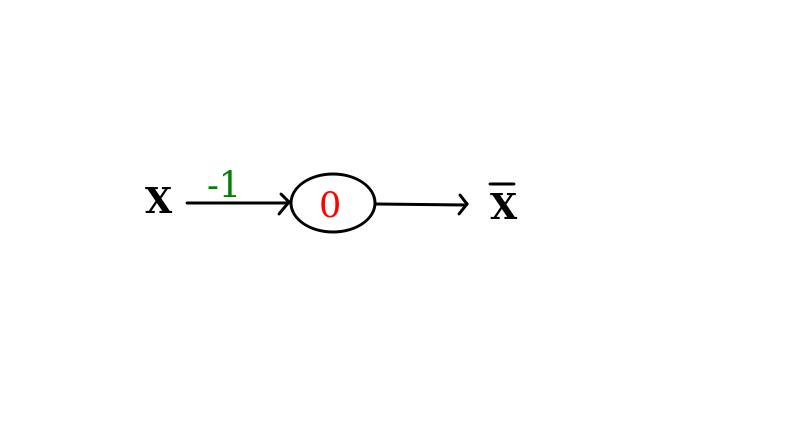
\includegraphics[scale=0.6]{negate2}
%\end{center}


\begin{figure}
\begin{tikzpicture}
\draw[blue,ultra thick]  (3,0) circle (20pt);
\foreach \y in {0}
  \draw[->] (0,\y) -- (2.3,0);
\foreach \y/\x in{0/$X$}
  \node[left] at (0,\y) {\x};

\foreach \y/\x in{0/$-1$}
  \node[above,orange] at (0+0.9,\y-0.5) {\x};

\draw[->] (3.7,0) -- (5,0);

\node[right,brown] at (5,0) {$\overline{X}$};
\node[red] at (3,0) {$0$};
\end{tikzpicture}
\end{figure}

\[
\overline{X}=\left \{ \begin{array}{ll}
1 &\mbox{if }-X\geq 0\\
0 &\mbox{else}
\end{array}
\right.
\]
\end{frame}



\begin{frame}
\frametitle{Majority Gate}
%\begin{center}
%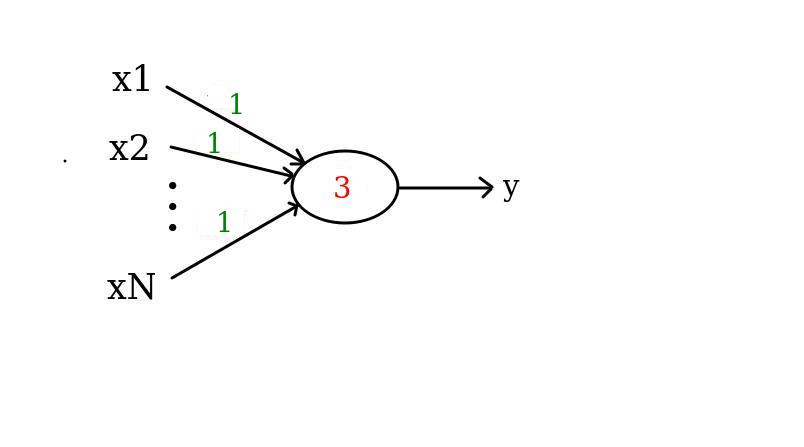
\includegraphics[scale=0.5]{three}
%\end{center}
\begin{figure}
\begin{tikzpicture}
\draw[blue,ultra thick]  (3,0) circle (10pt);
\foreach \y in {2,1,0,-2}
  \draw[->] (0,\y) -- (2.65,0);
\foreach \y/\x in{2/$x_1$,1/$x_2$,0/$x_3$,-2/$x_n$}
  \node[left] at (0,\y) {\x};

\foreach \y/\x in{2/$1$,1.1/$1$,0/$1$,-1.5/$1$}
  \node[above,orange] at (0+0.9,\y-0.5) {\x};
  
\node[left] at (0,-0.8) {$\vdots$};
\node[left] at (1,-0.6) {$\vdots$};

\draw[->] (3.35,0) -- (5,0);

\node[right,brown] at (5,0) {$y$};
\node[red] at (3,0) {$3$};
\end{tikzpicture}
\end{figure}


\[
y=\left \{ \begin{array}{ll}
1 &\mbox{if }\sum_{i=1}^nx_i\geq 3\\
0 &\mbox{else}
\end{array}
\right.
\]
\end{frame}


\begin{frame}
\frametitle{Universal AND Gate}
%\begin{center}
%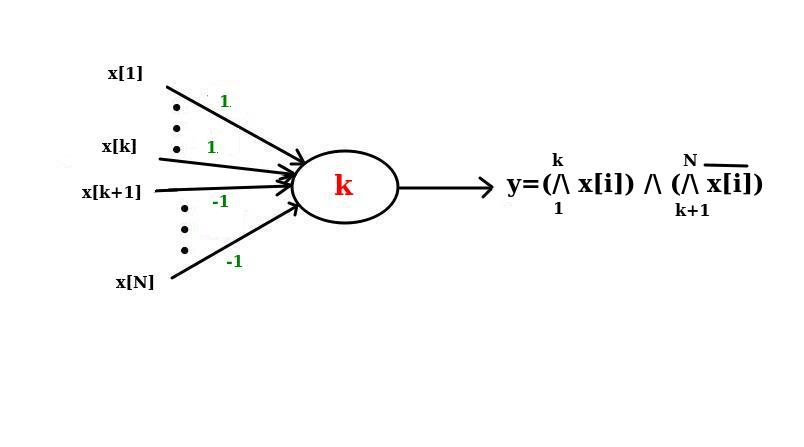
\includegraphics[scale=0.5]{univ_and}
%\end{center}
\begin{figure}
\begin{tikzpicture}
\draw[blue,ultra thick]  (3,0) circle (10pt);
\foreach \y in {2,1,0,-2}
  \draw[->] (0,\y) -- (2.65,0);
\foreach \y/\x in{2/$x_1$,1/$x_k$,0/$x_{k+1}$,-2/$x_n$}
  \node[left] at (0,\y) {\x};

\foreach \y/\x in{2/$1$,1.1/$1$,0/$-1$,-1.5/$-1$}
  \node[above,orange] at (0+0.9,\y-0.5) {\x};

\node[left] at (0,1.6) {$\vdots$};
\node[left] at (1,1.2) {$\vdots$};
  
\node[left] at (0,-0.8) {$\vdots$};
\node[left] at (1,-0.6) {$\vdots$};

\draw[->] (3.35,0) -- (5,0);

\node[right,brown] at (5,0) {$y=(\bigwedge_{i=1}^kx_i)\wedge(\bigwedge_{i={k+1}}^n\overline{x_i})$};
\node[red] at (3,0) {$k$};
\end{tikzpicture}
\end{figure}


\[
y=\left \{ \begin{array}{ll}
1 &\mbox{if }\sum_{i=1}^kx_i-\sum_{i=k+1}^nx_i\geq k\\
0 &\mbox{else}
\end{array}
\right.
\]
\end{frame}


%-----------


\begin{frame}
%\begin{center}
%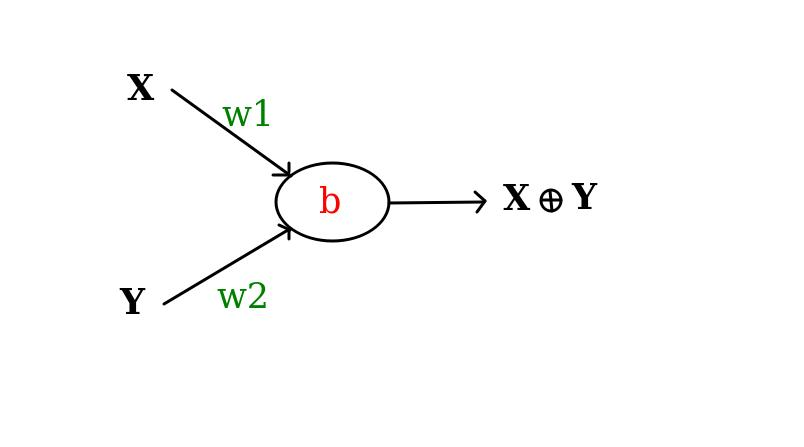
\includegraphics[scale=0.6]{xor}
%\end{center}

\begin{figure}
\begin{tikzpicture}
\draw[blue,ultra thick]  (3,0) circle (20pt);
\foreach \y in {2,-2}
  \draw[->] (0,\y) -- (2.3,0);
\foreach \y/\x in{2/$X$,-2/$Y$}
  \node[left] at (0,\y) {\x};

\foreach \y/\x in{2/$w_1$,-1.5/$w_2$}
  \node[above,orange] at (0+0.9,\y-0.5) {\x};

\draw[->] (3.7,0) -- (5,0);

\node[right,brown] at (5,0) {$X\oplus Y$};
\node[red] at (3,0) {$b$};
\end{tikzpicture}
\end{figure}

\[
X \oplus Y=\left \{ \begin{array}{ll}
1 &\mbox{if }w_1X+w_2Y\geq b\\
0 &\mbox{else}
\end{array}
\right.
\]
\end{frame}

\begin{frame}
\[
\begin{aligned}
& 1\oplus 0 =1 \Rightarrow w_1\geq b\\
& 0\oplus 1=1 \Rightarrow w_2\geq b\\
& 1\oplus 1=0 \Rightarrow w_1+w_2<b\\
& 0\oplus 0=0 \Rightarrow 0<b
\end{aligned}
\]
Find integers $w1, w_2, b$ that satisfies all of these constraints.
\end{frame}


\begin{frame}
\begin{figure}
\begin{tikzpicture}[thick,fill opacity=.3,draw opacity=3]
\draw[->] (0,-1) -- (0,5);
\draw[->] (-5,0) -- (5,0);
\node[right] at (5,0) {$w_1$};
\node[left] at (0,5) {$w_2$};
\draw[red,dotted] (-1,3) -- (3,-1);
\node[left] at (0,2) {$b$};
\node[below] at (2,0) {$b$};
\draw[fill=pink,fill opacity=.8, draw=none,rotate around={-45*5:(3,-1)}] (3,-1) rectangle (8,5);\pause

\draw[fill=green, draw=none] (-1,2) rectangle (8,6);
\draw[] (-1,2)-- (6,2); \pause
\draw[fill=green, draw=none] (2,-1) rectangle (6,7);
\draw[] (2,-1)-- (2,6); \pause
\node[above] at (2,2) {$(b,b)$};
%\draw[dotted, fill=blue] (2,0) -- (2,2) -- (0,2) -- cycle;
%\draw[] (2,0) -- (0,2);\pause
%\node[below] at (1,1) {$(1,1)$};
%\fill[] (1,1) circle [radius=2pt];
\end{tikzpicture}
\end{figure}
\end{frame}

%\begin{frame}
%\begin{center}
%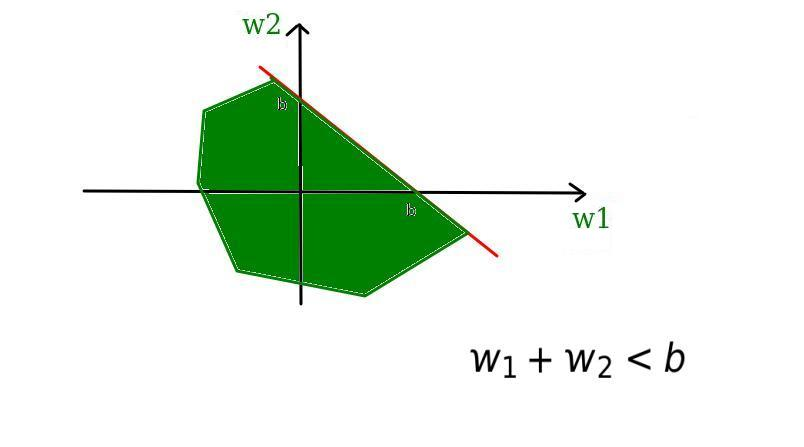
\includegraphics[scale=0.6]{xor3}
%\end{center}
%\end{frame}
%
%\begin{frame}
%\begin{center}
%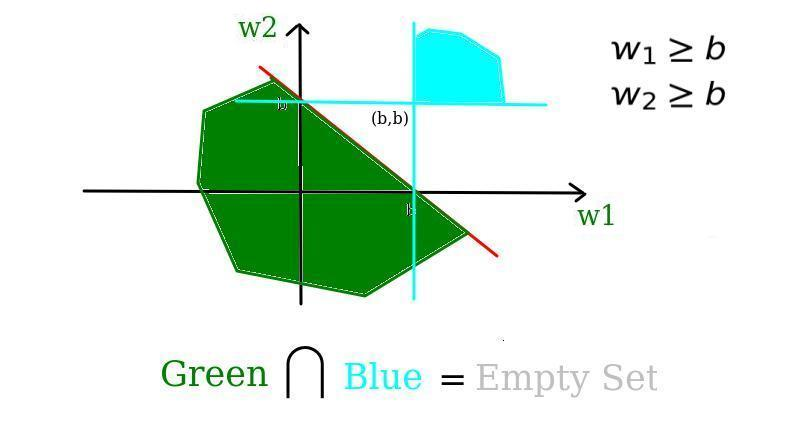
\includegraphics[scale=0.6]{xor4}
%\end{center}
%\end{frame}

\begin{frame}
\frametitle{Perceptron}
\begin{itemize}
\item Input $(x_1,\dots,x_N)$
\smallskip
\item Weights $(w_1,\dots,w_N)$  
\smallskip
\item If $w_1x_1+\dots+w_nx_n\geq b$ then output=1
\smallskip
\item Else, i.e., $w_1x_1+\dots+w_nx_n< b$, output=0
\end{itemize}
 
\end{frame}

\begin{frame}
%\begin{center}
%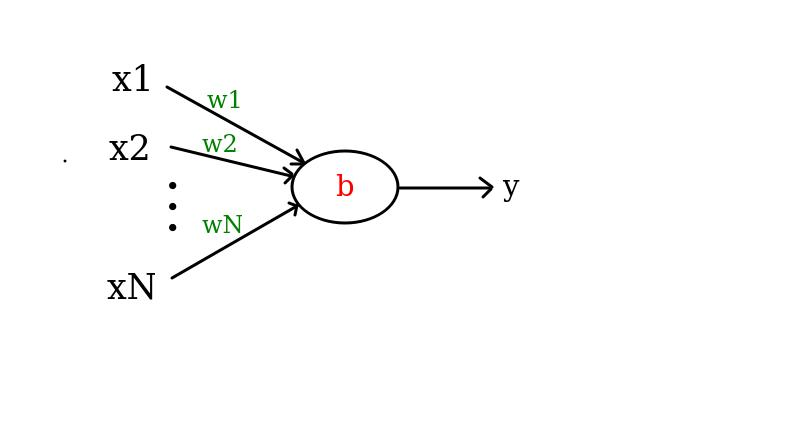
\includegraphics[scale=0.6]{perceptron}
%\end{center}

\begin{figure}
\begin{tikzpicture}
\draw[blue,ultra thick]  (3,0) circle (10pt);
\foreach \y in {2,1,0,-2}
  \draw[->] (0,\y) -- (2.65,0);
\foreach \y/\x in{2/$x_1$,1/$x_2$,0/$x_3$,-2/$x_n$}
  \node[left] at (0,\y) {\x};

\foreach \y/\x in{2/$w_1$,1.1/$w_2$,0/$w_3$,-1.5/$w_n$}
  \node[above,orange] at (0+0.9,\y-0.5) {\x};
  
\node[left] at (0,-0.8) {$\vdots$};
\node[left] at (1,-0.6) {$\vdots$};

\draw[->] (3.35,0) -- (5,0);

\node[right,brown] at (5,0) {$y$};
\node[red] at (3,0) {$b$};
\end{tikzpicture}
\end{figure}

\[
y=\left \{ \begin{array}{ll}
1 &\mbox{if }w_1x_1+\dots+w_Nx_N\geq b\\
0 &\mbox{else}
\end{array}
\right.
\]
\end{frame}

\begin{frame}
Let,
\[
\phi(z)=\left \{ \begin{array}{ll}
1 &\mbox{if }z\geq 0\\
0 &\mbox{else}
\end{array}
\right.
\]
then,
\[
y=\phi(w_1x_1+\dots+w_Nx_N-b)
\]
$\phi$ is called the \textbf{activation function}.
\end{frame}

\begin{frame}
\frametitle{Activation Functions}
\begin{itemize}
\item Identity: $\phi(z)=z$
\bigskip
\item Rectified linear unit (ReLU): $\phi (z)=max\{0,z\}$
\bigskip
\item Sigmoid: $\phi(z)=\frac{1}{1+e^{-z}}$
\bigskip
\item Hyperbolic tangent: $\phi(z)=\frac{e^z-e^{-z}}{e^z+e^{-z}}$
\bigskip
\item Binary step: $
\phi(z)=\left \{ \begin{array}{ll}
1 &\mbox{if }z\geq 0\\
0 &\mbox{else}
\end{array}
\right.
$
\end{itemize}
\end{frame}




\begin{frame}{}
  \centering \Huge
  \emph{Thank You}
\end{frame}

\end{document}

